\subsection{Classification on the dataset}
The group decided to analyse the data with a decision tree, $K$ nearest neighbour and an artificial neural network. Furthermore a two level cross validation was used for selecting parameters, a 10-fold was used for both outer and inner fold. \newline


\subsubsection{Decision Tree}
The parameters for the decision tree was based off a tree depth ranging from 1-20. Below (figure \ref{fig:classification_boxplot}.) shows a boxplot for the optimal levels for each fold. 

\vspace{-5pt}
\begin{figure}[!ht]
	\centering
	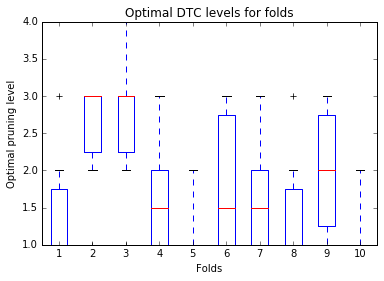
\includegraphics[width=0.7\textwidth]{Fig/classification_decision_tree}
	\vspace{-5pt}
	\caption{Boxplot for the decision tree}
	\label{fig:classification_boxplot}
\end{figure}

\subsubsection{Artificial Neural Network}
The artificial neural network was trained with 5 networks per fold, with at 10 fold cross validation. The network gave a good low test error rate at 6.88955955862\%. Below is the result of the ANN illustrated.

\vspace{-5pt}
\begin{figure}[!ht]
	\centering
	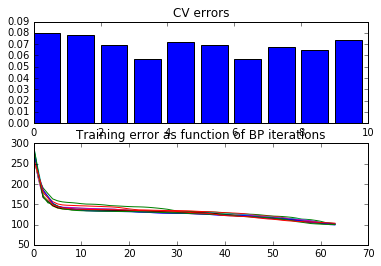
\includegraphics[width=0.6\textwidth]{Fig/classification_ANN_1}
	\vspace{-5pt}
	\caption{Errors for each fold of the ANN}
	\label{fig:classification_ANN}
\end{figure}

\vspace{-5pt}
\begin{figure}[!ht]
	\centering
	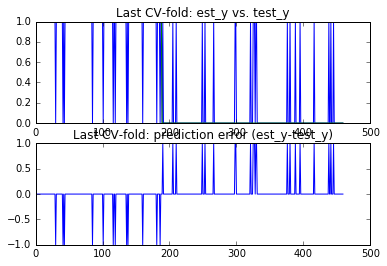
\includegraphics[width=0.6\textwidth]{Fig/classification_ANN_2}
	\vspace{-5pt}
	\caption{Comparing estimated values and test values, from the ANN}
	\label{fig:classification_ANN2}
\end{figure}

\newpage
\subsubsection{K-Nearest Neighbour}
The K-Nearest Neighbour analysis was carried out in the same way as the decision tree, below (figure \ref{fig:classification_KNN}.) is the result of the analysis with KNN. The best error rate of the KNN analysis was 8.83459555812\%.

\vspace{-5pt}
\begin{figure}[!ht]
	\centering
	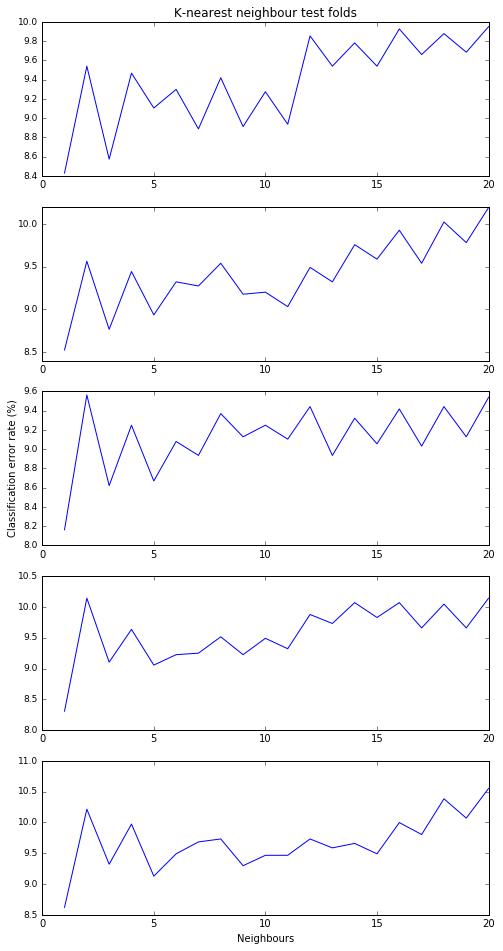
\includegraphics[width=0.7\textwidth]{Fig/classification_KNN}
	\vspace{-5pt}
	\caption{K-Nearest Neighbour error for each fold}
	\label{fig:classification_KNN}
\end{figure}

\subsubsection{Comparing the K-Nearest Neighbour with the Artificial Neural Network}
For comparing the two best preforming methods a series of t-test have been carried out on the result for each method. The t-value of the test was 5.4900656372629992 and the p-value was 0.00038510731768533901. With the result of the t-test, the Artificial Neural Network is the preferred method for the classification problem on the dataset. 